\documentclass[pdf, hyperref={unicode}, aspectratio=169]{beamer}
\setbeameroption{hide notes}
% \setbeameroption{show only notes}

\usepackage{styles}

\title{Разреженная идентификация нелинейных динамических систем}

\subtitle{Выпускная квалификационная работа бакалавра}

\pdfstringdefDisableCommands{
  \def\\{}
  \def\,{}
  \def\textbf#1{<#1>}
}

\author[Бирюков Виктор Владимирович]
{
  \textbf{Студент группы М8О-407Б-19:} Бирюков Виктор Владимирович\\
  \ \textbf{Научный руководитель:} д.ф.-м.н., проф., проф. каф. 806 Д.\,Л.\,Ревизников
}

\institute[Московский авиационный институт]
{
  Московский авиационный институт (национальный исследовательский университет)\\
  Институт № 8 «Компьютерные науки и прикладная математика»\\
  Кафедра № 806 «Вычислительная математика и программирование» 
}

\date{Москва --- \the\year}

\logo{
\includegraphics[height=1cm]{img/mai}}

\begin{document}

{
% убирает номер слайда с титульного слайда
\setbeamertemplate{page number in head/foot}{}
\frame{\titlepage}
}


\begin{frame}
\frametitle{Актуальность темы}

\begin{itemize}
  \item Динамические системы описывают большое количество различных процессов.
  \item Задача извлечения закономерностей из большого объема данных может превышать возможности человека.
  \item Знание динамической системы, лежащей за данными, позволит использовать соответствующий математический аппарат как часть анализа данных.
\end{itemize}

\note{
Актуальность данной темы связана с тем, что при помощи динамических систем можно описать очень большое количество различных процессов.
Динамические системы могут иметь различную природу, например, это могут быть обыкновенные дифференциальные уравнения, дифференциальные уравнения в частных производных или рекуррентные соотношения.

Таким образом может возникать задача по извлечению закономерностей в виде динамической системы из данных, которые описывают некоторый процесс.
Однако, если данные имеют большой объем, такая задача может быть непосильна человеку.
Именно поэтому необходим алгоритм, который способен это сделать.

Знание динамической системы, лежащей за данными, также может помочь в анализе данных, так как появляется возможность использовать методы анализа самой системы. 
}
\end{frame}


\begin{frame}
\frametitle{Цель и задача работы}

\textbf{Цель} --- идентификация систем обыкновенных дифференциальных уравнений на основе зашумленных данных.

\textbf{Задачи:}
\begin{itemize}
  \item Реализация алгоритма идентификации.
  \item Реализация алгоритмов дифференцирования шумных данных.
  \item Реализация алгоритмов разреженной регрессии.
  \item Тестирование алгоритма идентификации на известных системах ОДУ. Сравнение различных методов.
\end{itemize}

\note{
Таким образом цель работы --- идентификация систем обыкновенных дифференциальных уравнений на основе зашумленных данных.

Задачи --- реализация самого алгоритма идентификации, а также реализация его составных частей --- алгоритмов дифференцирования шумных данных и алгоритмов разреженной регрессии, и, наконец, тестирование алгоритма на известных системах обыкновенных дифференциальных уравнений и сравнение между собой различных методов дифференцирования и регрессии.
}
\end{frame}


\begin{frame}
\frametitle{Постановка задачи}

\textbf{Дано:}
\begin{itemize}
  \item Входные данные представляют из себя массив значений некоторых величин
  \item Данные могут содержать некоторую шумовую компоненту
  \item Предполагается, что замеры величин производились через равные промежутки времени
\end{itemize}

\textbf{Необходимо} разработать алгоритм, при помощи которого можно получить динамическую систему (систему ОДУ), которая описывает эволюцию заданных величин.

\note{
Соответственно, входные данные представляют из себя массив значений некоторых величин. 
Эти данные могут содержать некоторую шумовую компоненту.
И предполагается, что что замеры величин производились через равные промежутки времени
}
\end{frame}


\begin{frame}
\frametitle{Алгоритм решения задачи}

\begin{figure}
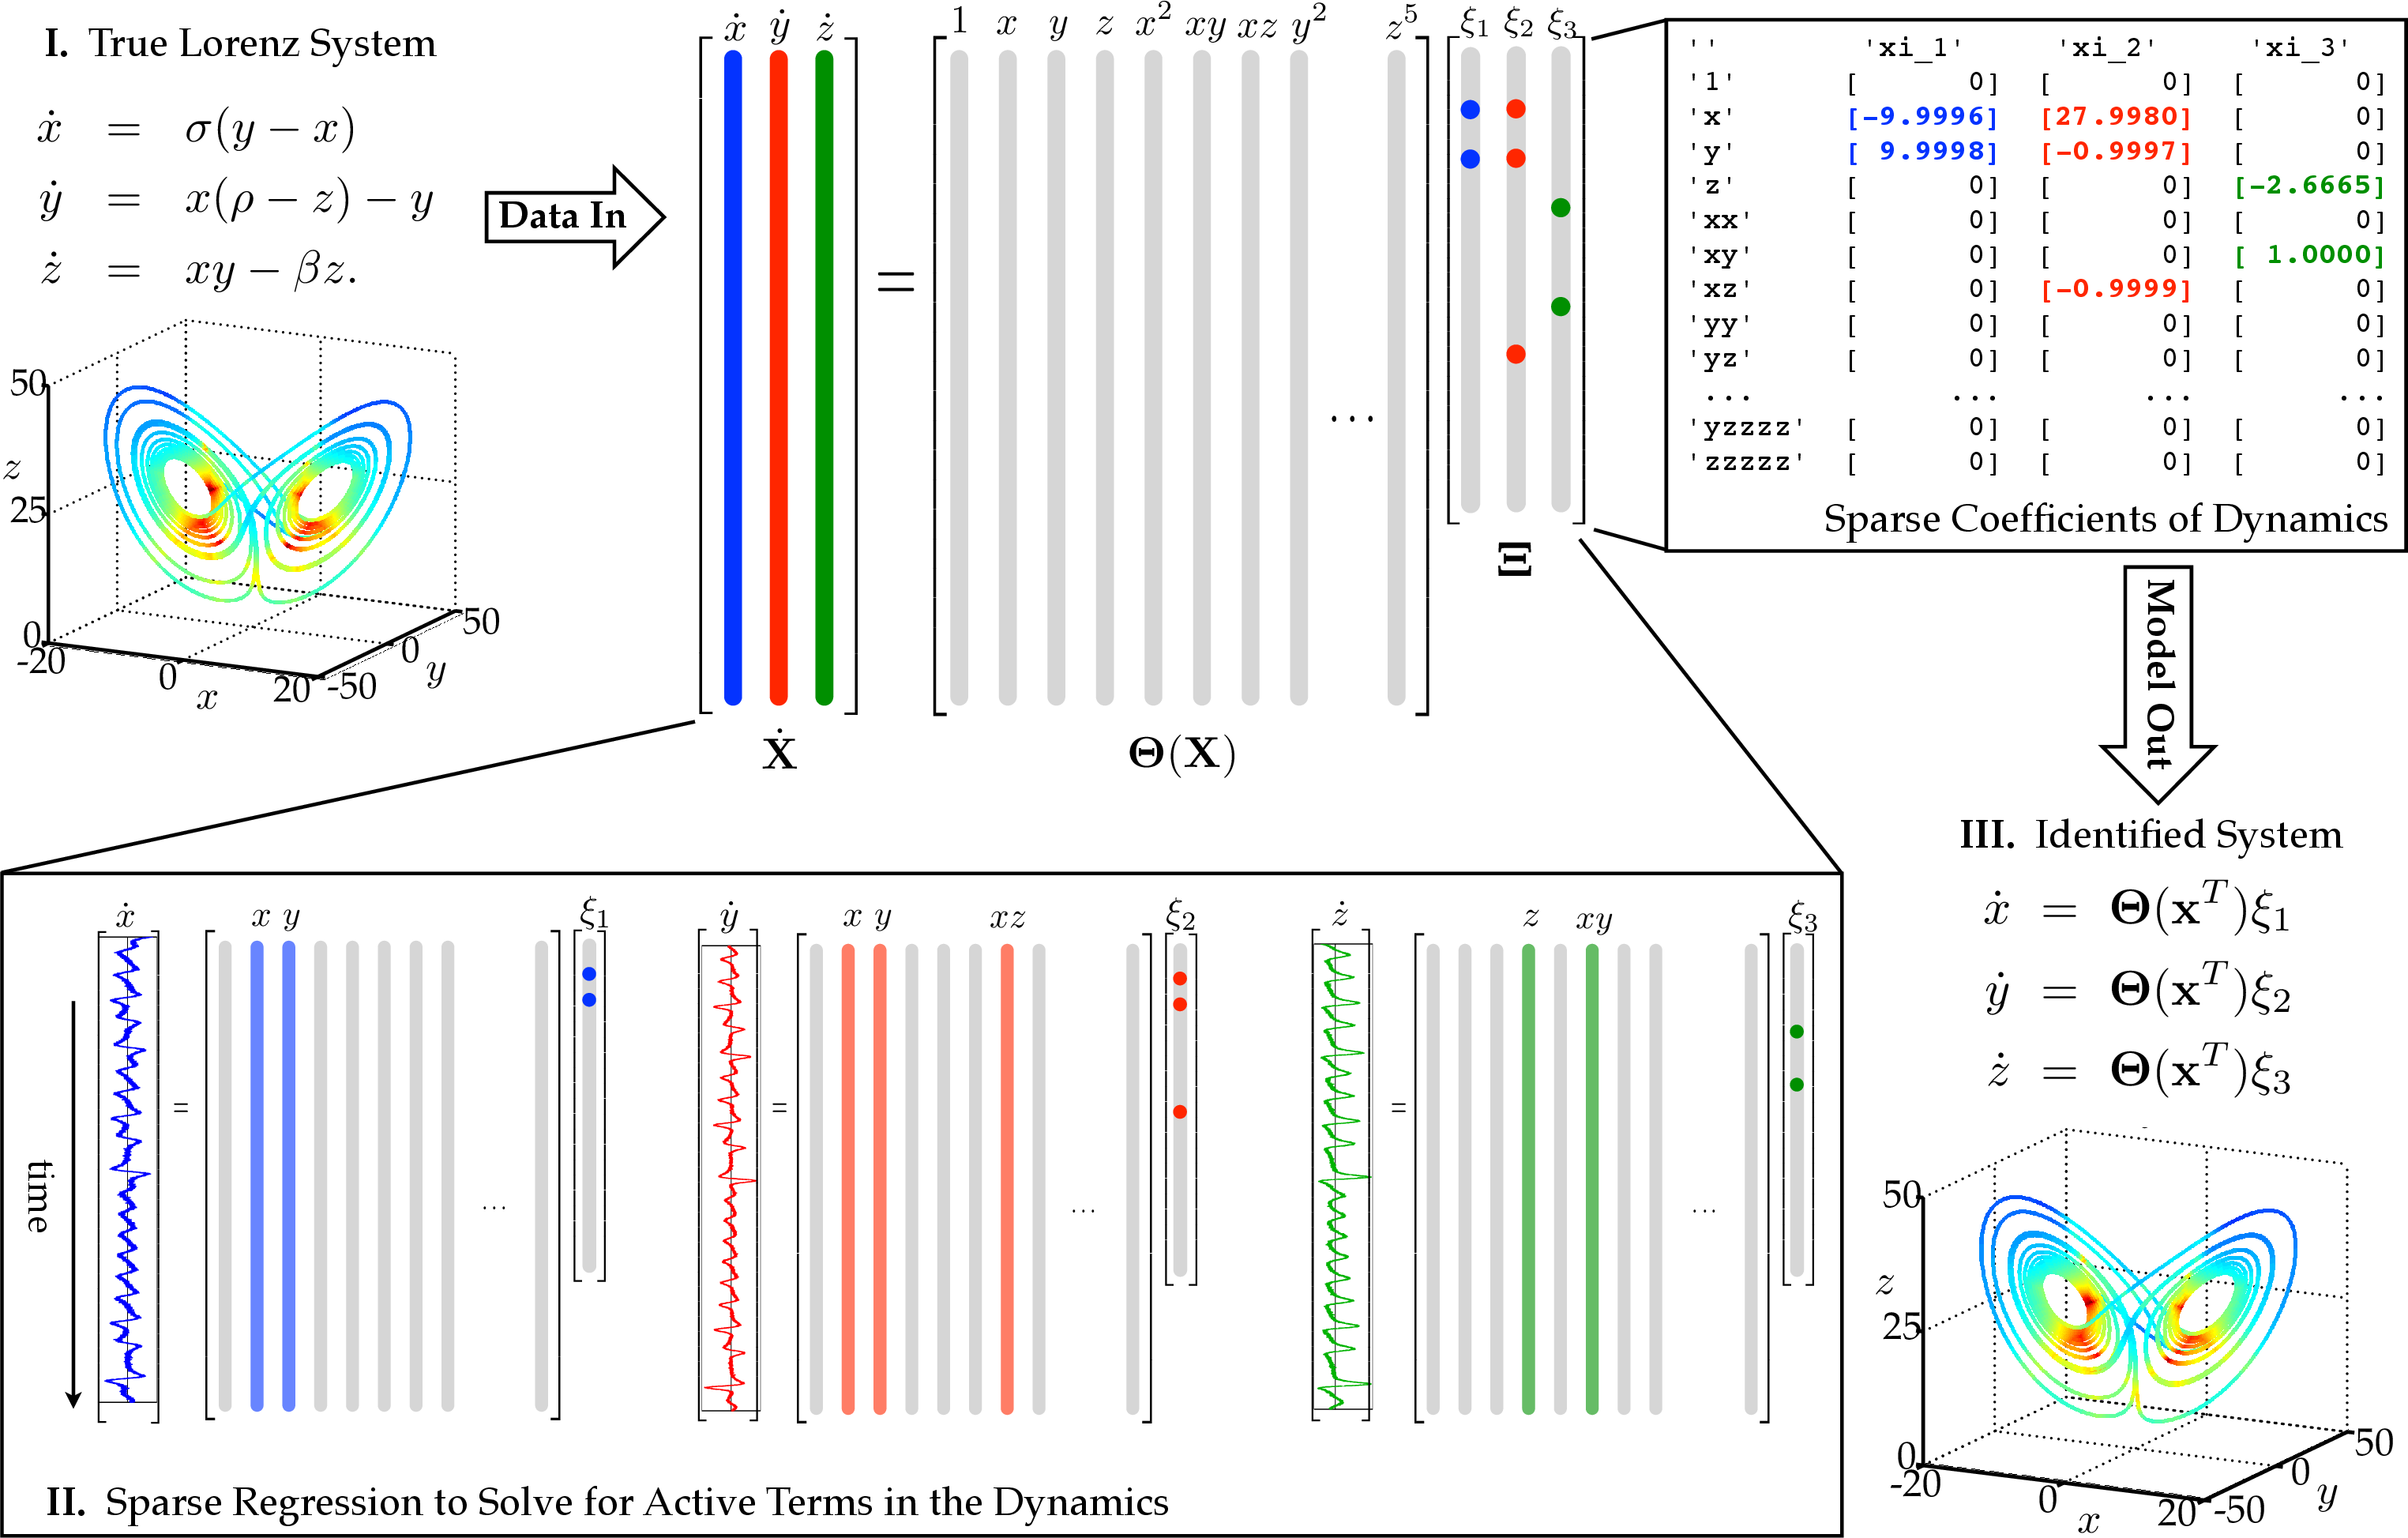
\includegraphics[height=0.78\textheight]{img/sindy_scheme}
\caption{\scriptsize\hfill Brunton et al., 2016}
\end{figure}

\note{
\footnotesize
Алгоритм идентификации представляет из себя следующее. Каждое из обыкновенных дифференциальных уравнений системы представляет из себя зависимость между производной одной величины и комбинацией некоторых величин. Комбинация в общем случае нелинейная, однако заметим, что очень часто правая часть уравнения содержит довольно мало слагаемых, и эти слагаемые довольно простые.

Например, здесь изображена система Лоренца, и правые части этой системы содержат полиномиальные комбинации величин, причем их степень не превышает вторую.

Таким образом, для заданных измерений величин, можно использовать алгоритм численного дифференцирования для получения производных, и затем составить матрицу предполагаемых слагаемых правых частей theta(X). После этого можно решить задачу разреженной линейной регрессии между этими матрицами и получить разреженную матрицу коэффициентов ksi. Тогда столбец этой матрицы будет определять какие слагаемые входят в правую часть соответствующего уравнения. 

При этом даже будут получены коэффициенты при этих слагаемых, однако они будут не слишком точными, основной упор здесь делается именно на структурный анализ, а не на параметрический.
}
\end{frame}


\begin{frame}
\frametitle{Стек технологий}

\begin{itemize}
  \item Язык программирования Python
  \item Библиотеки научных вычислений NumPy и SciPy
  \item Библиотека машинного обучения Scikit-learn
  \item Библиотеки построения графиков Matplotlib и Seaborn
\end{itemize}

\note{
Что касается используемых технологий, то основной язык реализации --- Python, так как это очень удобный язык программирования для работы с данными.

В ходе реализации алгоритмов активно использовались библиотеки научных вычислений NumPy и SciPy, а сами алгоритмы используют инфраструктуру библиотеки машинного обучения Scikit-learn, которая предоставляет удобный набор базовых классов.

И, так как основной результат работы --- это графики различных функций, восстановленных систем, и так далее, для их построения использовалась библиотека Matplotlib.
}
\end{frame}


\begin{frame}
\frametitle{Архитектура решения}

Разработанное решение реализовано в формате модуля языка Python.
\begin{figure}
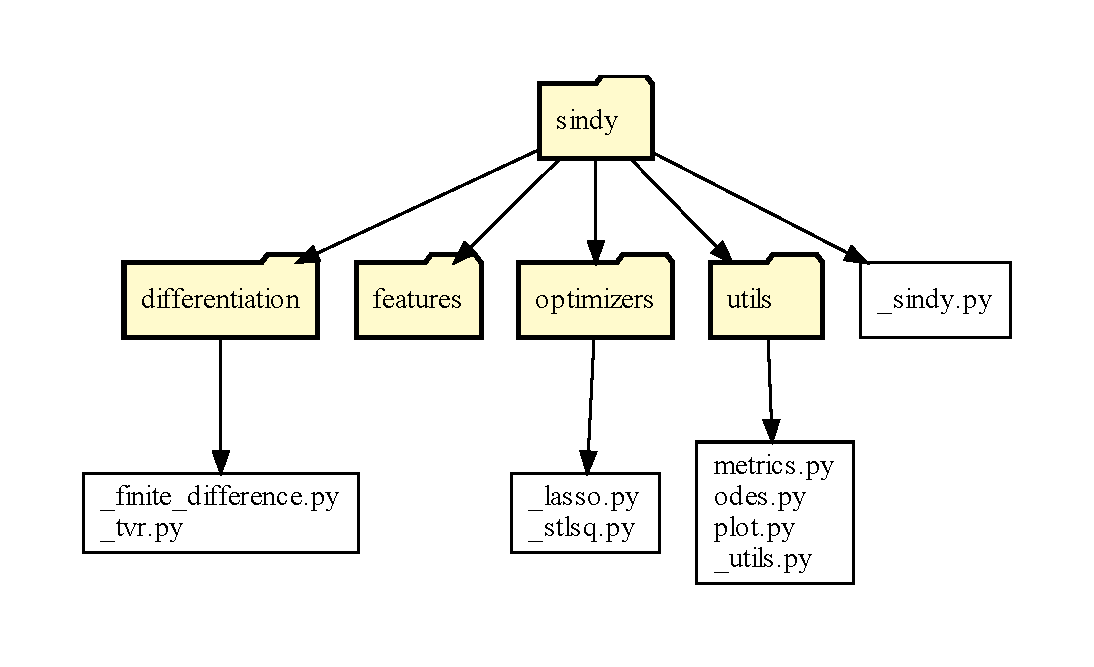
\includegraphics[height=0.8\textheight]{img/tree}
\end{figure}

\note{
Разработанное решение реализовано в формате модуля языка Python. Здесь можно видеть алгоритм идентификации, алгоритмы дифференцирования, регрессии, а также различные вспомогательные вещи --- метрики, использованные системы уравнений, функции для отрисовки графиков.
}
\end{frame}


\begin{frame}
\frametitle{Описание программной разработки}

Репозиторий с исходным кодом расположен по адресу \url{https://github.com/iktovr/bachelor-diploma}

\begin{figure}

\includegraphics[height=0.7\textheight]{img/qr-code}
\end{figure}

\end{frame}


\begin{frame}
\frametitle{Работа с данными}

В качестве источника данных использовались различные системы ОДУ:
\begin{figure}
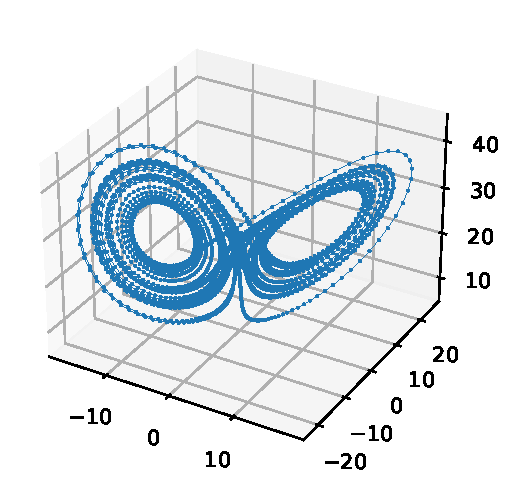
\includegraphics[height=0.38\textheight]{img/lorenz}\hfill
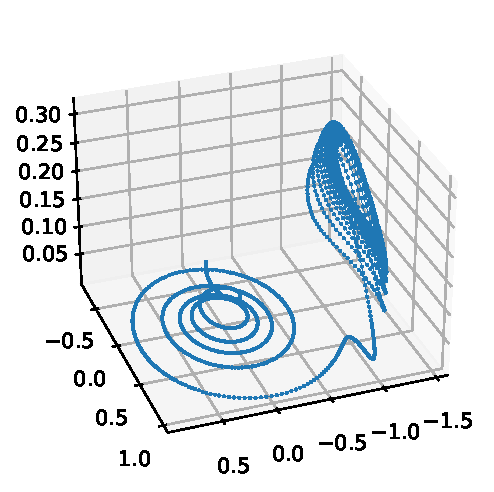
\includegraphics[height=0.38\textheight]{img/fabrab}\hfill
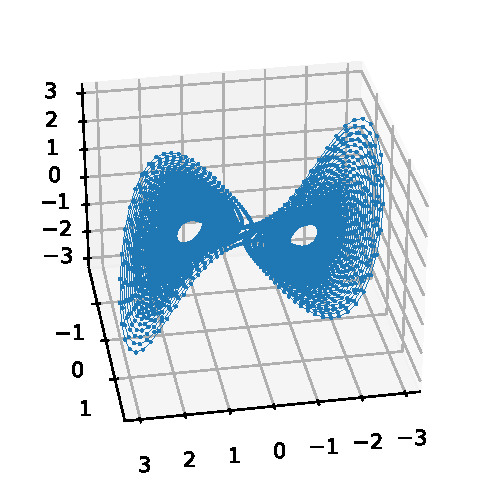
\includegraphics[height=0.38\textheight]{img/moore_spiegel}\hfill
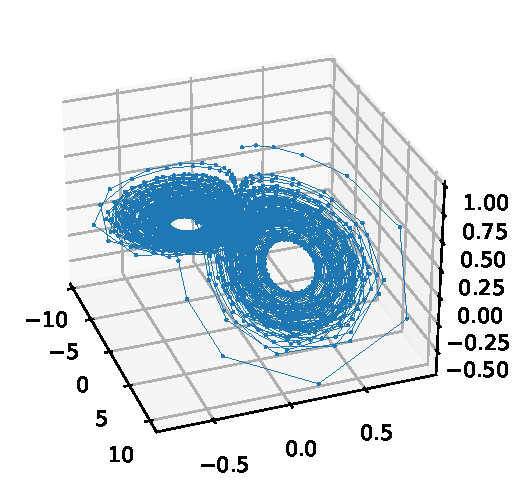
\includegraphics[height=0.38\textheight]{img/vallis}

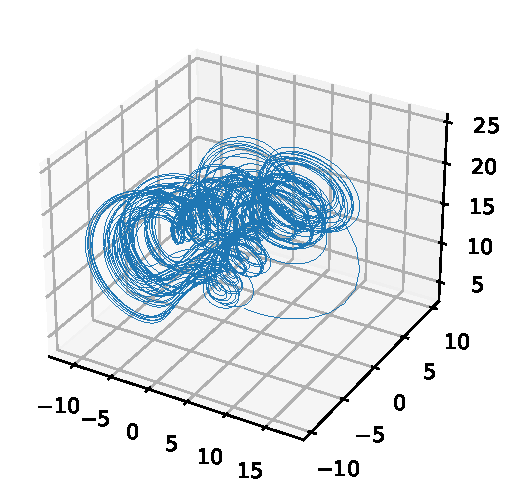
\includegraphics[height=0.38\textheight]{img/generator2}\hfill
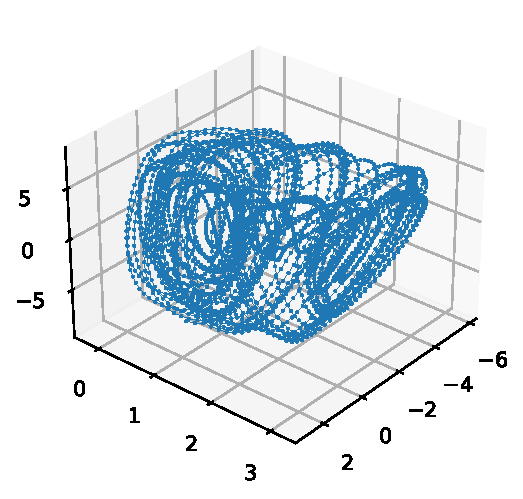
\includegraphics[height=0.38\textheight]{img/torus}\hfill
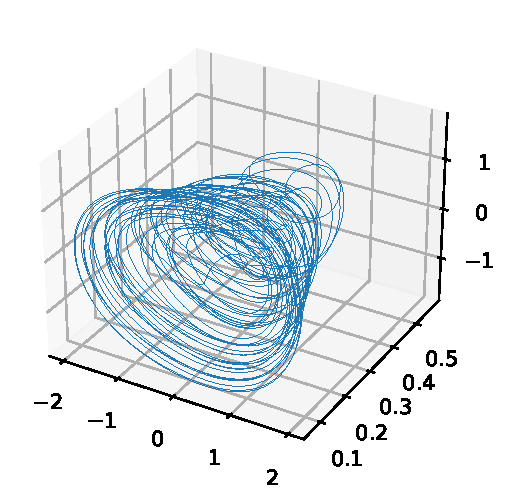
\includegraphics[height=0.38\textheight]{img/aritmic}\hfill
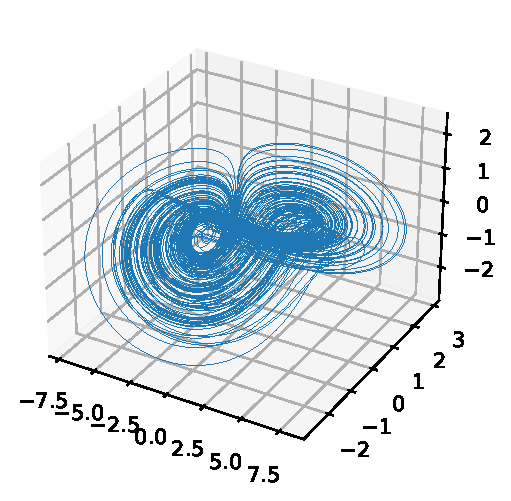
\includegraphics[height=0.38\textheight]{img/simple_3d_model}
\end{figure}

\note{
В качестве источника данных использовались различные системы ОДУ, в основном трехмерные. Так, в первом ряду можно видеть систему Лоренца, систему Фабриканта-Рабиновича, систему Мура-Шпигеля, систему Валлиса. Также использовались некоторые другие системы.
}
\end{frame}


\begin{frame}
\frametitle{Результаты разработки}

\framesubtitle<1-3>{Численное дифференцирование}
\begin{onlyenv}<1-3>
\begin{figure}
\includegraphics<1>[width=0.49\linewidth]{img/alpha_fast_tvr}\only<1>{\hfill}
\includegraphics<1>[width=0.49\linewidth]{img/alpha_tvr}
\includegraphics<2>[width=\textwidth]{img/sin_test}
\includegraphics<3>[height=0.75\textheight]{img/lorenz_test}
\end{figure}
\end{onlyenv}

\note<1>{
Важной частью работы стал анализ алгоритмов численного дифференцирования, так как, применительно к задаче идентификации, алгоритмы дифференцирования, основанные на регуляризации полной вариации ранее не применялись.

Поэтому были разработаны некоторые рекомендации по их использованию. Например, была обнаружена зависимость между уровнем шума в данных и оптимальным значением коэффициента регуляризации. А именно, порядок коэффициента регуляризации пропорционален уровню шума, графики показаны на слайде.
}

\note<2>{
Используя эти знания, можно довольно успешно дифференцировать функции при различном уровне шума. Здесь показан пример с синусоидой.
}

\note<3>{
И более сложный пример с аттрактором Лоренца. Видно, что, когда метод конечных разностей совершенно перестает работать, специализированные методы все еще выдают приемлемую производную, с относительно небольшой средней ошибкой.
}

\framesubtitle<4>{Разреженная регрессия}
\begin{onlyenv}<4>
\begin{figure}
\subfloat[Алгоритм Lasso]{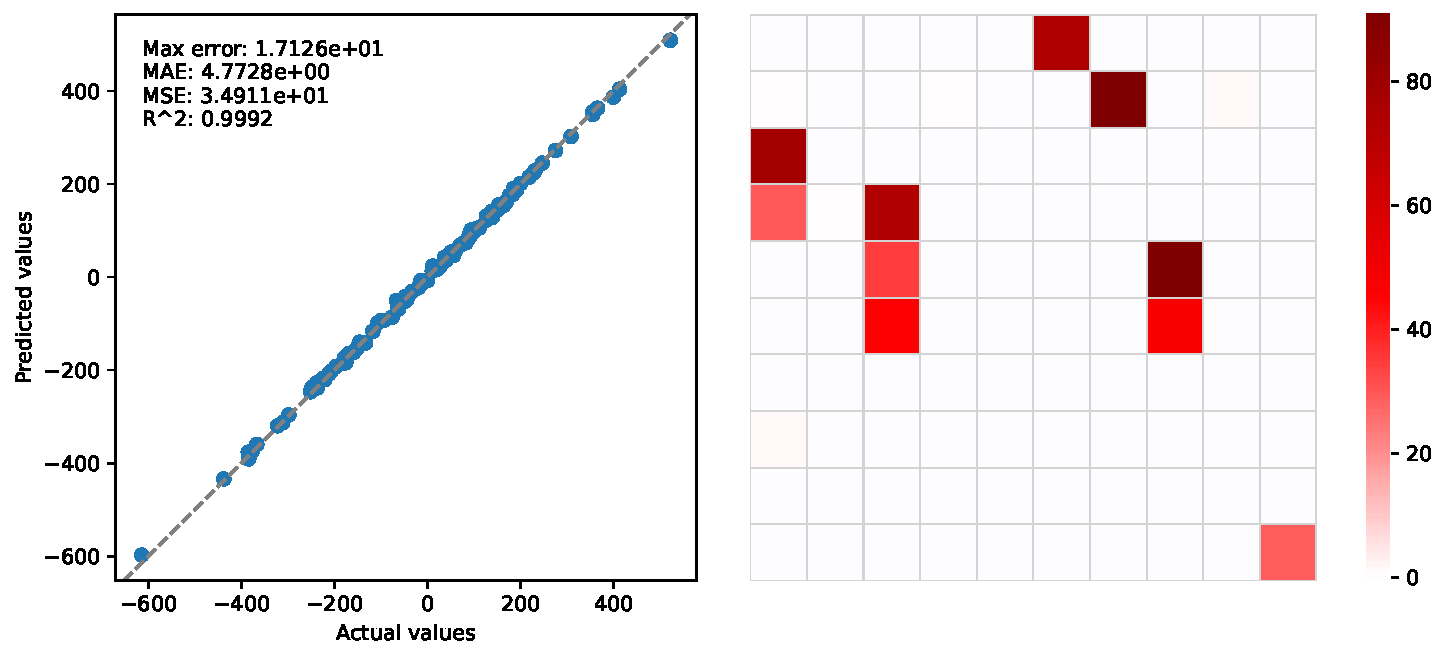
\includegraphics[width=0.49\linewidth]{img/lasso}}\hfill
\subfloat[Алгоритм STLSQ]{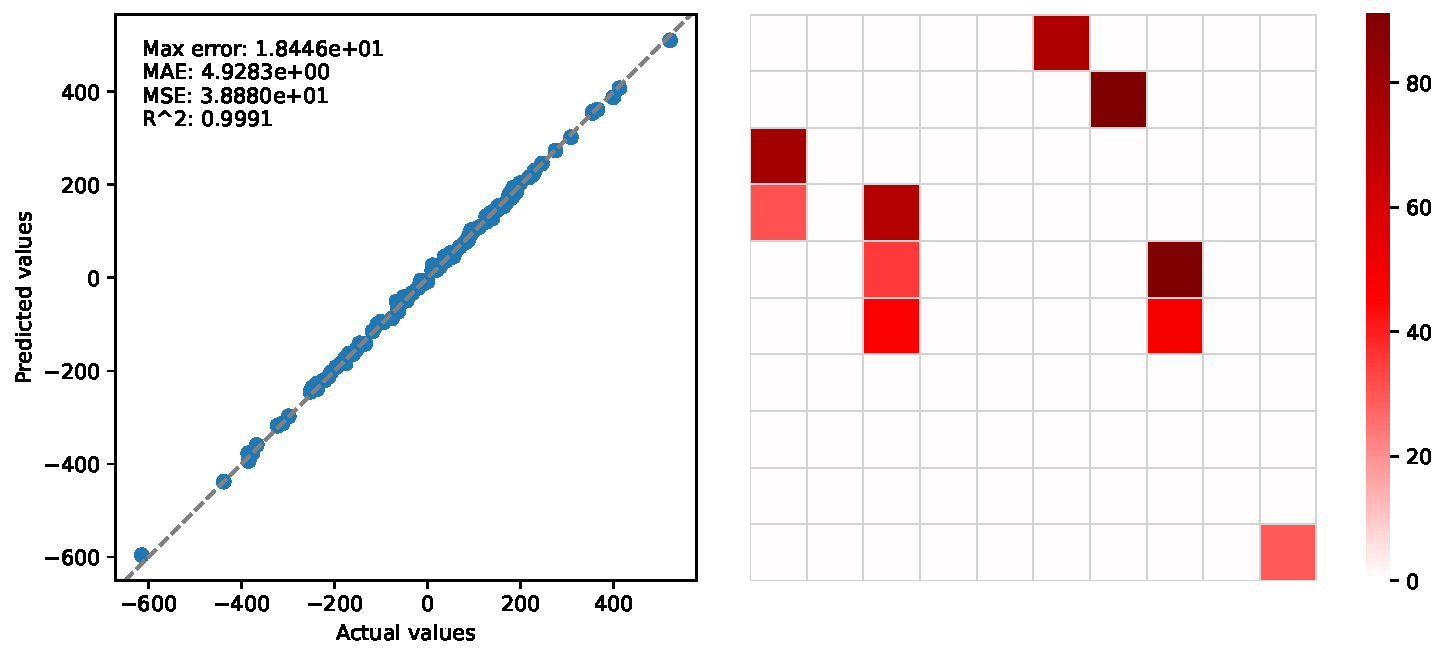
\includegraphics[width=0.49\linewidth]{img/stlsq}}
\end{figure}
\end{onlyenv}

\note<4>{
Также в работе использованы два алгоритма разреженной регрессии, это классический алгоритм машинного обучения Lasso, и новый алгоритм STLSQ. На рисунках изображен пример задачи регрессии со ста признаками, из которых только десять значимые.

Видно, что оба алгоритма справились с обнаружением этих десяти признаков, и сама задача регрессии решается довольно точно.
}

\framesubtitle<5>{Идентификация}
\begin{onlyenv}<5>
\begin{figure}
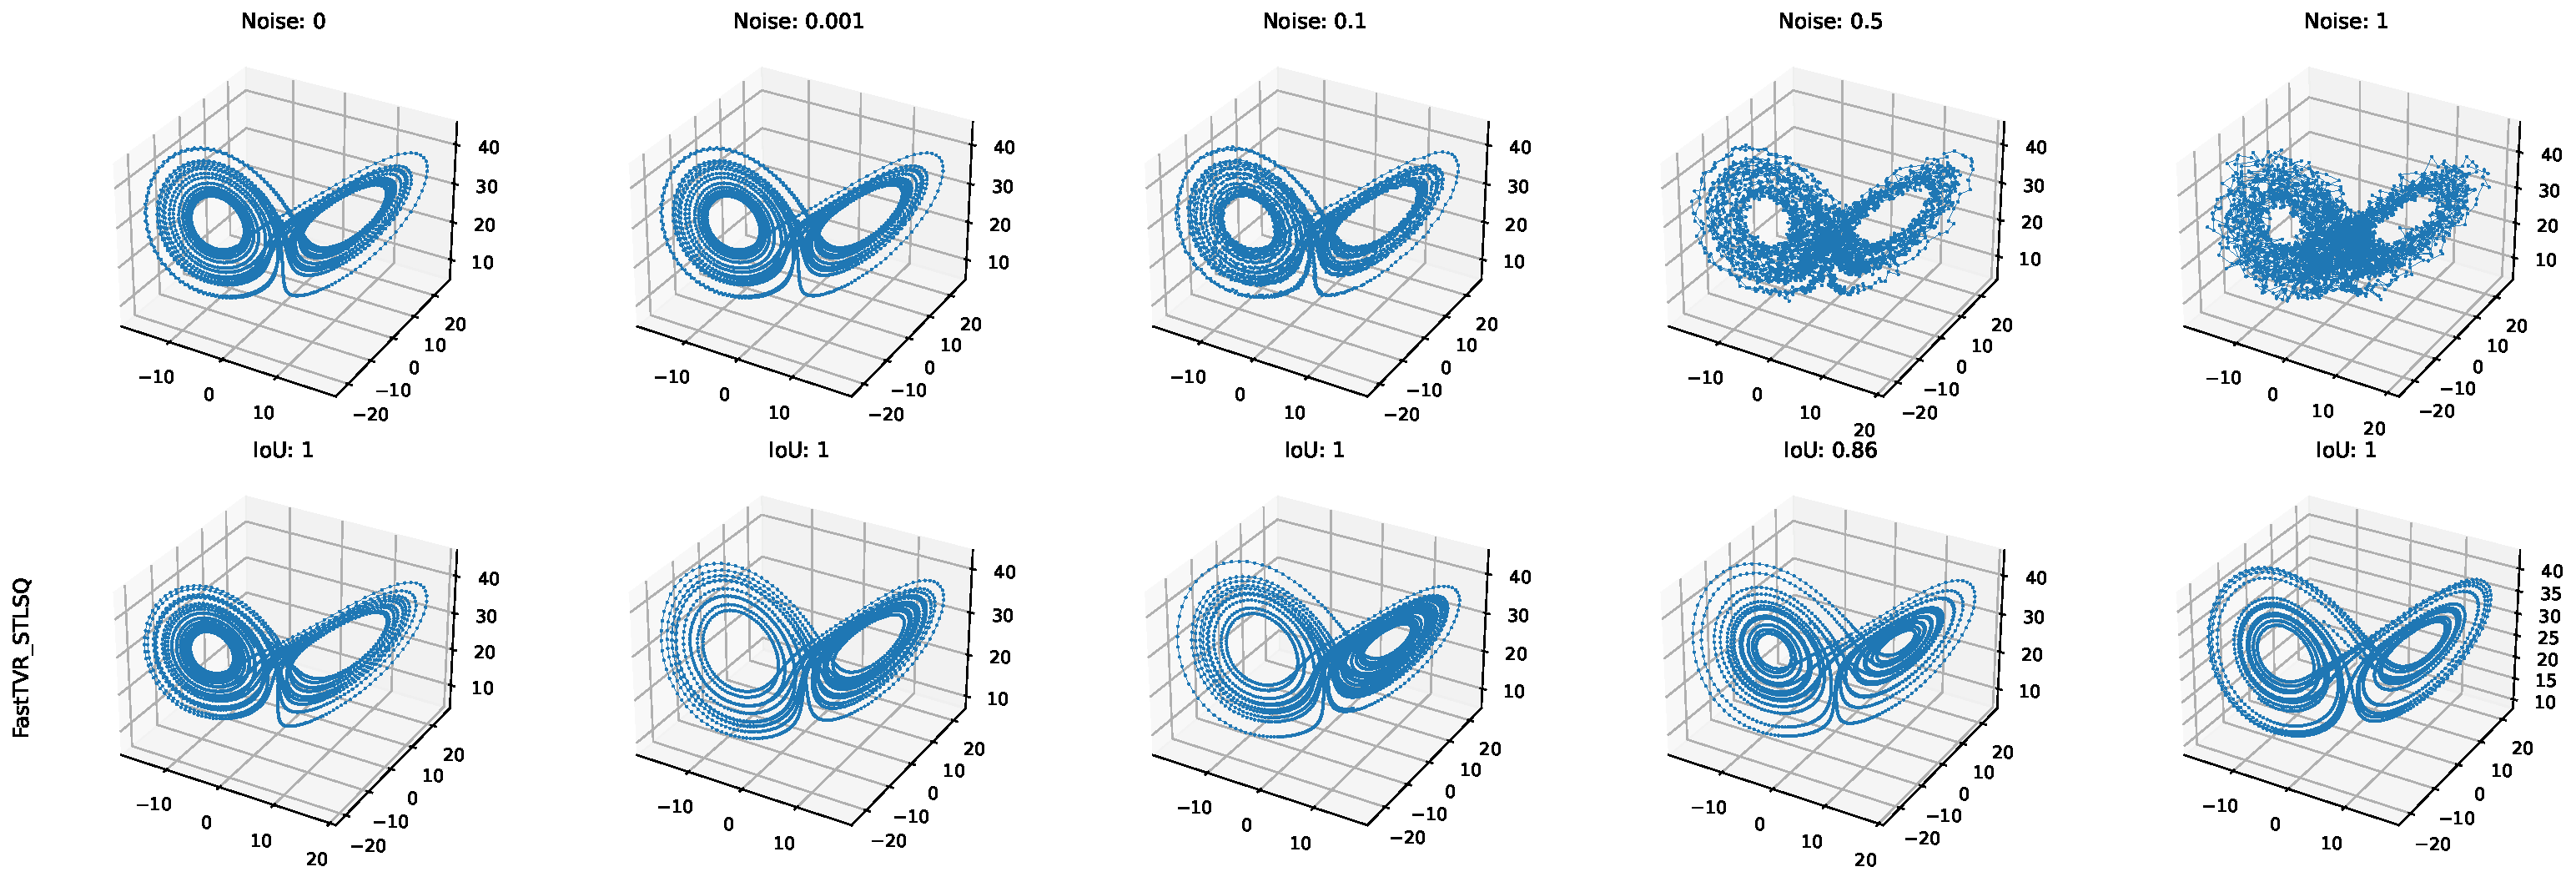
\includegraphics[width=\textwidth]{img/sindy_test}
\end{figure}
{\tiny\textcolor{lightgray}{(Здесь будет более подробное изображение)}}
\end{onlyenv}

\note<5>{
И, наконец, используя все описанные выше алгоритмы, можно решать задачу идентификации. На данном слайде представлен пример с системой Лоренца, видно, что практически при всех уровнях шума удалось добится значения метрики один. Это метрика intersection over union, она позаимствовал ее из задачи семантической сегментации, и в данном случае она обозначает то, какая часть из предсказанных слагаемых совпала с реальными слагаемыми.

При этом можно заметить, что восстановленные системы не очень похожи на оригинальную, это связано с тем, что коэффициентами восстанавливаются неточно, параметрическая идентификация является отдельной большой задачей.
}
\end{frame}


\begin{frame}
\frametitle{Оценка результата}

\begin{itemize}
\item Основной результат заключается в том, что идентификация систем ОДУ по шумным данным вполне осуществима.
\item Однако, для этого необходимо иметь подходящий набор функций предполагаемых слагаемых.
\item Для эффективной борьбы с шумом нужно также оценивать его величину.
\end{itemize}

\note{
В случае реальных данных, это можно делать, например, используя методы спектрального анализа.
}
\end{frame}


\begin{frame}
\frametitle{Отзывы и рецензия}

\begin{columns}
\column{0.5\textwidth}
\center{Скан отзыва научного руководителя}

\column{0.5\textwidth}
\center{Скан рецензии}
\end{columns}
\end{frame}

\end{document}
